\documentclass[12pt,t]{beamer}
\usepackage{graphicx}
\usepackage[vlined]{algorithm2e}
\usepackage{times}
\usepackage{calc}
\usepackage{url}
\usepackage{soul}
\usepackage{graphicx}
\usepackage{multirow, hhline}
\usepackage{array, booktabs, colortbl}
\usepackage{amsmath}
\usepackage{amssymb}
\usepackage{relsize}
\usepackage{multirow}
\usepackage{booktabs}
\usepackage{pagecolor}
\usepackage{lipsum}
\usepackage{capt-of}
\usepackage{booktabs}

\usepackage{graphicx}
\usepackage{multicol}
\usepackage[T1]{fontenc}
\usepackage{ae}
\graphicspath{{fig/}}
\setbeameroption{hide notes}
\setbeamertemplate{note page}[plain]

\usetheme{default}
\beamertemplatenavigationsymbolsempty
\hypersetup{pdfpagemode=UseNone}

\usefonttheme{professionalfonts}
\usefonttheme{serif}
\usepackage{fontspec}
\setmainfont{Karla}
\setbeamerfont{note page}{family*=pplx,size=\footnotesize} % Palatino for notes

\definecolor{foreground}{RGB}{70,70,70}
\definecolor{background}{RGB}{249, 249, 249} %24,24,24
%\definecolor{title}{RGB}{107,174,214} %107,174,214
\definecolor{title}{RGB}{70,70,70}
\definecolor{gray}{RGB}{0,0,0}
\definecolor{subtitle}{RGB}{70,70,70}
\definecolor{hilight}{RGB}{102,255,204}
\definecolor{vhilight}{RGB}{255,111,207}
\definecolor{Gray}{gray}{0.85}
\definecolor{LiteGray}{gray}{0.92}

\setbeamercolor{titlelike}{fg=title}
\setbeamercolor{subtitle}{fg=subtitle}
\setbeamercolor{institute}{fg=gray}
\setbeamercolor{normal text}{fg=foreground,bg=background}


\setbeamercolor{item}{fg=foreground} % color of bullets
\setbeamercolor{subitem}{fg=gray}
\setbeamercolor{itemize/enumerate subbody}{fg=gray}
\setbeamertemplate{itemize subitem}{{\textendash}}
\setbeamerfont{itemize/enumerate subbody}{size=\footnotesize}
\setbeamerfont{itemize/enumerate subitem}{size=\footnotesize}

\setbeamercolor{block title}{fg=white,bg=gray!70}
\setbeamercolor{block body}{fg=black,bg=gray!10}
\setbeamercolor{block title alerted}{fg=red,bg=gray!40}
\setbeamercolor{block title example}{fg=black,bg=green!20}
\setbeamercolor{block body example}{fg=black,bg=green!5}
\setbeamerfont{block title}{series=\bfseries}

\hypersetup{colorlinks,linkcolor=foreground,urlcolor=foreground}


\setbeamertemplate{footline}{%
    \raisebox{5pt}{\makebox[\paperwidth]{\hfill\makebox[20pt]{\color{gray}
          \scriptsize\insertframenumber}}}\hspace*{5pt}}

\addtobeamertemplate{note page}{\setlength{\parskip}{12pt}}


\newcommand{\bi}{\begin{itemize}}
\newcommand{\ei}{\end{itemize}}
\newcommand{\ig}{\includegraphics}
\newcommand{\subt}[1]{{\footnotesize \color{subtitle} {#1}}}

\let\emph\relax % there's no \RedeclareTextFontCommand
\DeclareTextFontCommand{\emph}{\bfseries\em}

\def\imagetop#1{\vtop{\null\hbox{#1}}}

\setbeamertemplate{frametitle}
{\vskip4pt
  \leavevmode
%\hbox{%
\begin{beamercolorbox}[wd=\paperwidth,ht=2ex,dp=0ex]{frametitle}%
\underline{\makebox[\paperwidth][l]{\hspace*{10pt}
\large {{\insertframetitle}}}}
\end{beamercolorbox}
%  }%
}

%\setbeamercolor{frametitle}{fg=yellow,bg=red}

\begin{document}

\AtBeginSection[]{
  \begin{frame}
  \vfill
  \centering
  \begin{beamercolorbox}[sep=8pt,center,shadow=true,rounded=true]{title}
    \underline{\makebox[0.8\paperwidth][l]{
\large {{\insertsectionhead}}}}
  \end{beamercolorbox}
  \vfill
  \end{frame}
}

\title{\large{Workshop \#1: Introduction to Python for Data Science}}
\subtitle{TRiCAM 2017}
\author{W. Pan}
%\institute{Harvard University}
\date{}
\titlegraphic{
   
\includegraphics[height=2cm]{iacs}
\includegraphics[height=2cm]{harvard}
\includegraphics[height=2cm]{hogwarts}
}
{
\setbeamertemplate{footline}{} % no page number here
\frame{
  \titlepage
  
}
}

\begin{frame}{Lecture Outline}
\tableofcontents
\end{frame}

%%%%%%%%%%%%%%%%%%%%%%%%%%%%%%%%%%%%%%%%%%%%%%%%%%%%%%%%%%%%%%%%%%%%%%%%%%%%%%
\section{Review}

\begin{frame}{The Data Science Process} 
Recall the Data Science Process we outlined yesterday:
\vskip0.2cm
\begin{itemize}
\item Ask questions
\item  Data Collection
\item  Data Exploration
\alert{\item  Data Modeling}
\alert{\item  Data Analysis}
\item  Visualization and Presentation of Results 
\end{itemize}
\vskip0.2cm
Yesterday we addressed data collection and exploration. Today we'll be addressing building models for data and analyzing the results.
\end{frame}

\begin{frame}{Data Collection: Summary} 
\vskip-0.4cm
A couple of important observations from yesterday:
\begin{itemize}
\item Real world data can be a mess. It can have:
\begin{itemize}
\item missing values (requires data imputation)
\item erroneous values (requires outlier detection)
\item inconsistent or non-comparable units (requires rescaling, normalization or standardization)
\item messy format (require reformatting)
\end{itemize}
\item Real word data can be hard to get. Limitations include:
\begin{itemize}
\item expensive API
\item no API, requires scraping
\item is not digitized
\item very old, or not old enough
\end{itemize}
\end{itemize}
\textbf{Motto:} Data scientists put data first! Be vigilant for any potential weakness in the integrity of your data and be will to spend substantial creative energy on data gathering/processing alone.
\end{frame}

\begin{frame}{Data Exploration: Summary} 
A couple of important observations from yesterday:
\begin{itemize}
\item \textbf{Basic intuition:} shape of data (no. of observations, dimension of feature space), types of variables (quantitative vs categorical).
\item \textbf{Descriptive statistics:} summarizing the values 
\begin{itemize}
\item \textbf{`typical value':} mean or median for quantitative, mode for categorical
\item \textbf{`spread':} range, variance/standard deviation, quantiles
\end{itemize}
\item \textbf{Data visualization:} qualitatively exploring relationships and trends
\begin{itemize}
\item \textbf{Distribution:} histogram for single variable, scatter plot for multiple variables
\item \textbf{Relationships:} scatter plot, trend line
\item \textbf{Composition:} pie chart, bar chart, stacked area graph
\item \textbf{Comparisons:} multiple trends or histograms in one chart
\end{itemize}
\end{itemize}
\end{frame}

\begin{frame}{Try It Yourself!}
Apply what you've learned about the data science process to explore a SoCal real-estate listings data set!
\end{frame}

%%%%%%%%%%%%%%%%%%%%%%%%%%%%%%%%%%%%%%%%%%%%%%%%%%%%%%%%%%%%%%%%%%%%%%%%%%%%%%
\section{Motivating Regression}
\begin{frame}{Californian Home Prices (2009)}
\begin{tabular}{lp{5.5cm}}
\only<1-2>{\imagetop{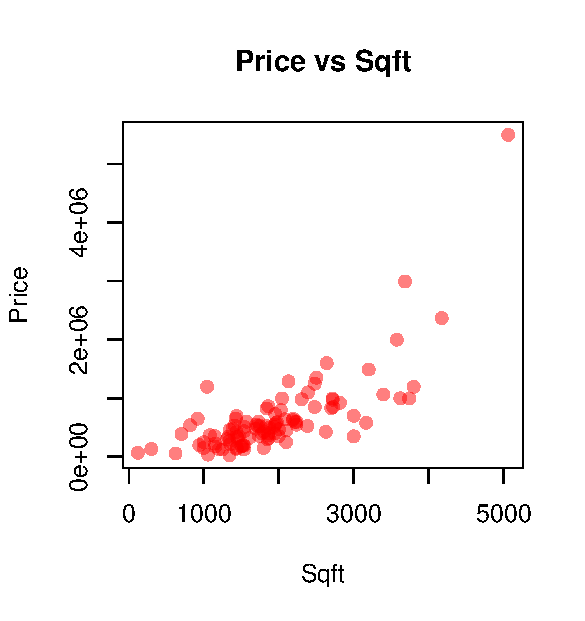
\includegraphics[height=50mm]{scatter}} & 
\begin{enumerate}
\only<1>{\item[]This is a scatter plot of home prices vs square footage of some homes in southern California. 
\vskip0.2cm
\item[]Can you see any patterns or trends?}
\only<2>{\item[] We see that \textbf{as square footage increases, so does price}. 
\vskip0.2cm
\item[] But what is a precise, mathematical description of this relationship?}
\end{enumerate}
}
\only<3>{\imagetop{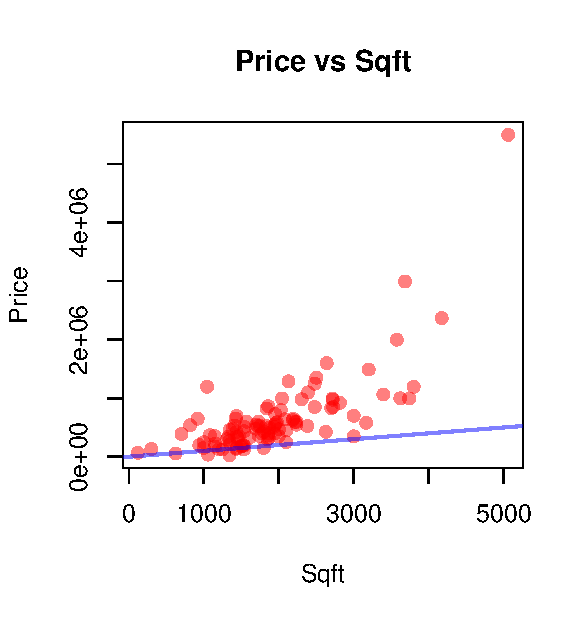
\includegraphics[height=50mm]{line1}} & 
\begin{enumerate}
\item[]Maybe we want to model the relationship between square footage and price using a simple line. 
\vskip0.2cm
\item[]Does this line capture the trend in the data?
\end{enumerate}
}
\only<4>{\imagetop{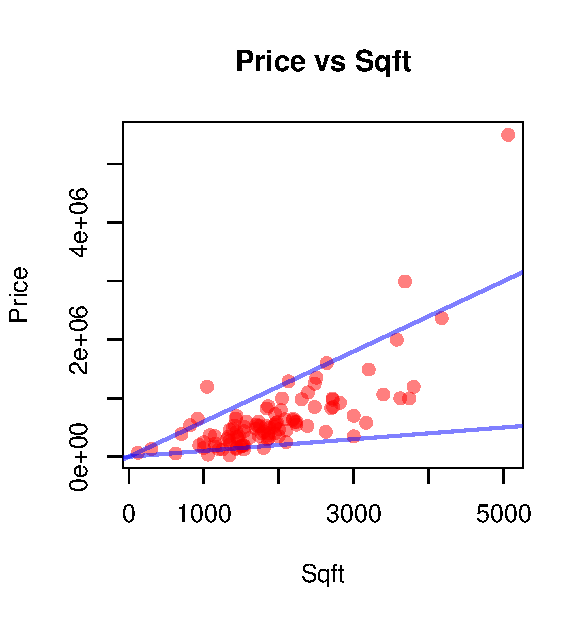
\includegraphics[height=50mm]{line2}} & 
\begin{enumerate}
\item[]What about this line?
\end{enumerate}
}
\only<5>{\imagetop{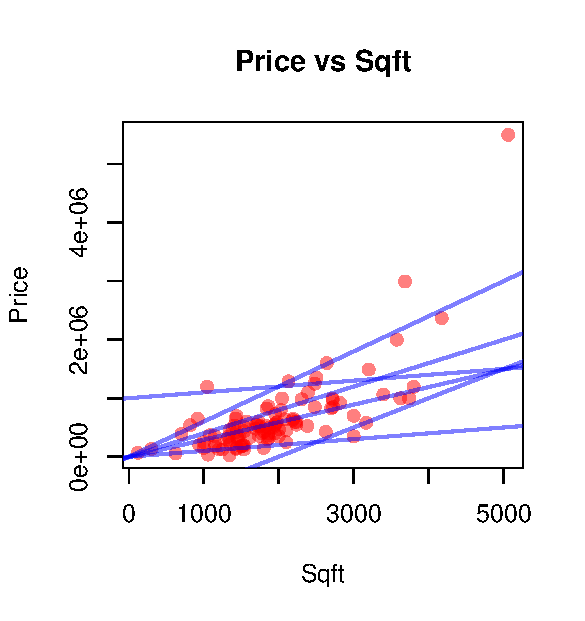
\includegraphics[height=50mm]{line3}} & 
\begin{enumerate}
\item[]In fact, there are infinite number of lines we can draw through the data. 
\vskip0.2cm
\item[] Which is the best line?
\vskip0.2cm
\item[]What is a good definition for `\emph{the best line}'?
\end{enumerate}
}
\end{tabular}
\end{frame}

\begin{frame}{Notion of Error}
\begin{tabular}{lp{5.5cm}}
\imagetop{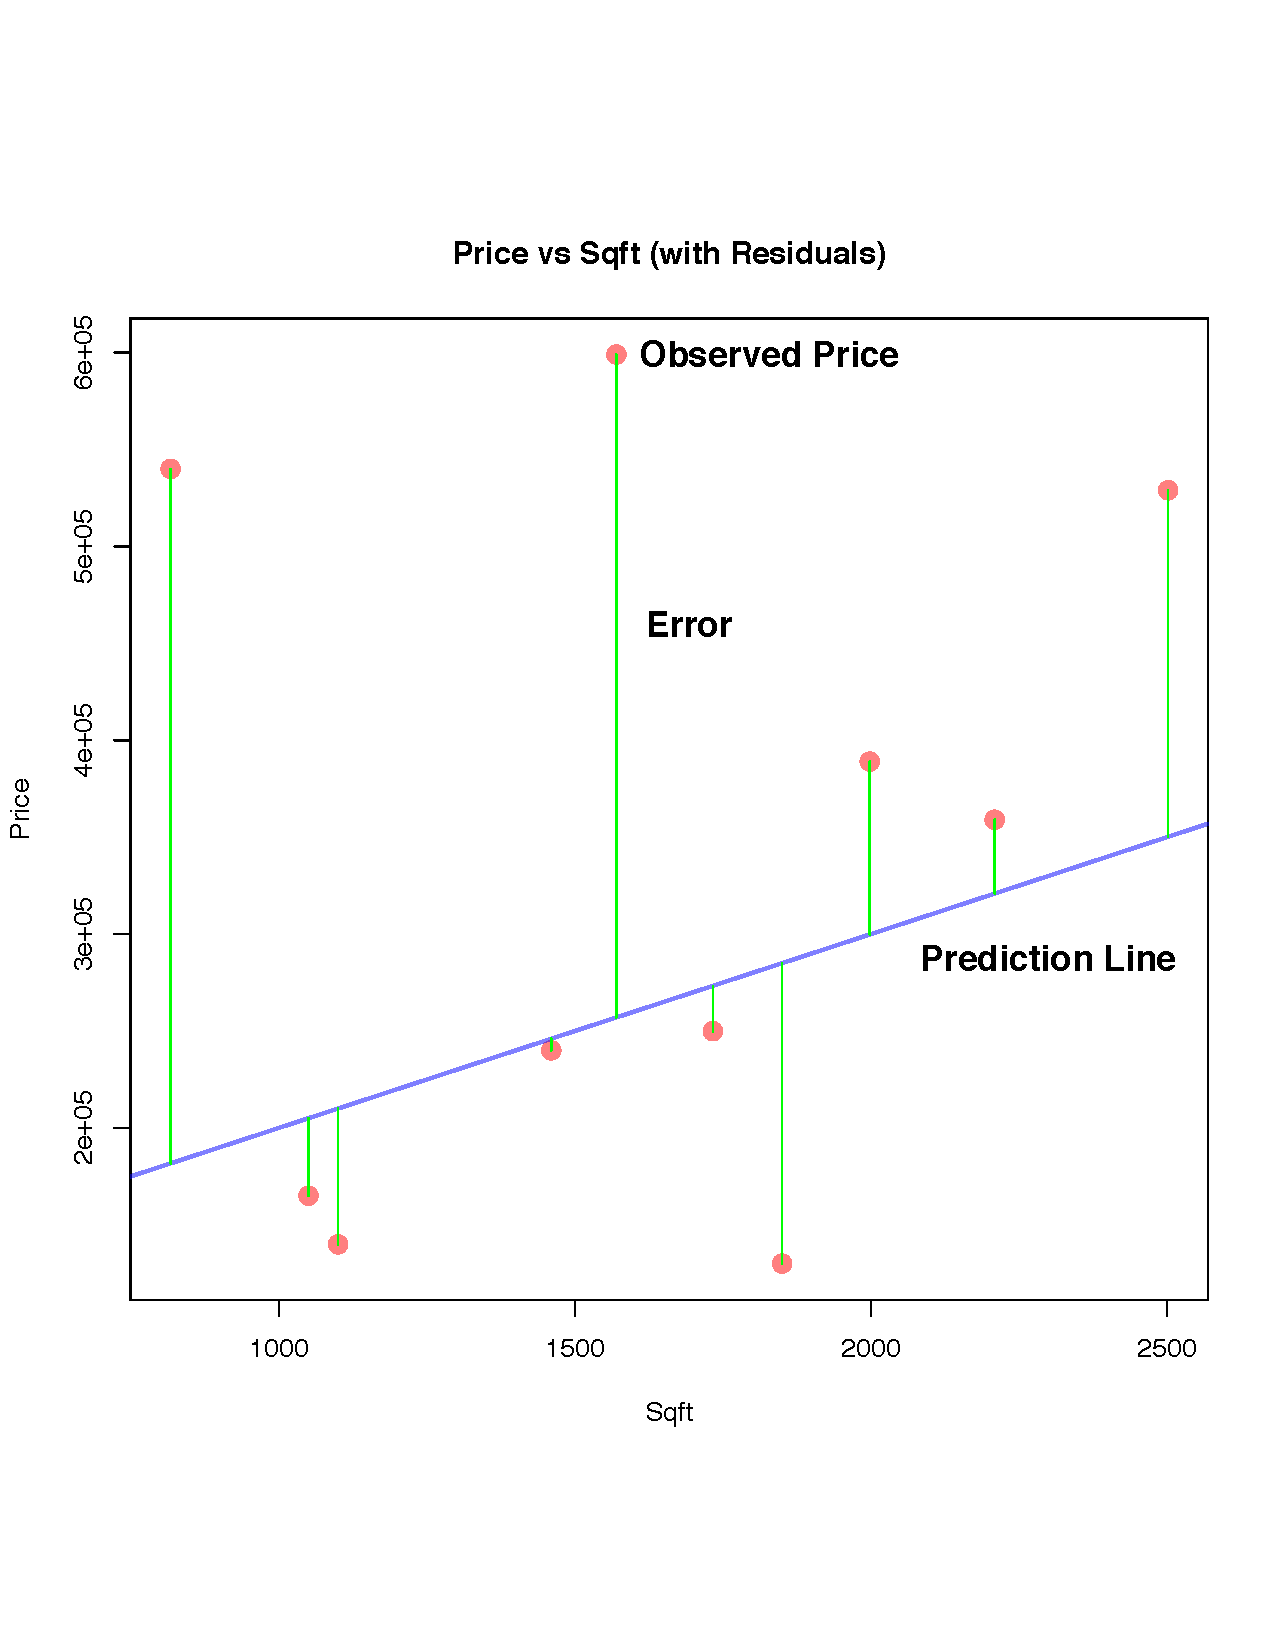
\includegraphics[height=50mm]{residuals}} & 
\begin{enumerate}
\only<1>{\item[] An \emph{absolute residual} is the absolute difference between the actual price of a home and the price predicted by the line for a given square footage.
\[
\text{\scriptsize Res}_i = |\text{\scriptsize Observed}_i - \text{\scriptsize Predicted}_i|
\]
}
\only<2>{\item[] The $i$-th absolute residual measures the magnitude of the `error' made by the $i$-th prediction.}

\end{enumerate}
\end{tabular}
\vskip0.4cm

\end{frame}

\begin{frame}{Notions of Fitness}
\vskip-0.4cm
\textbf{Question:} How do we quantify the overall error?
\vskip0.2cm
\begin{enumerate}
\item (\textbf{Max absolute deviation}) Count only the biggest `error'
\[
\max_i |\mathrm{Observed}_i - \mathrm{Predicted}_i| 
\]
\item (\textbf{Sum of absolute deviations}) Add up the `errors'
\[
\sum_i |\mathrm{Observed}_i - \mathrm{Predicted}_i| 
\]
We can also average them.
\item (\textbf{Sum of squared errors}) Add up the squares of the `errors'
\[
\sum_i |\mathrm{Observed}_i - \mathrm{Predicted}_i|^2 
\]
We can also average them.
\end{enumerate}
\end{frame}

%Fitting/Predicting
\begin{frame}{Model Fitting}
\vskip-0.4cm
\textbf{Question:} What do we mean by choosing `the best line'?
\vskip0.2cm
\textbf{Answer:} A line which minimizes the overall error.
\vskip0.2cm
\only<1>{\textbf{Example:} Given a set of points $(x_1, y_1), \ldots, (x_n, y_n)$, the \textbf{average of absolute deviations} of a line $y = mx + b$ is 
\[
L(m, b) = \frac{1}{n} \sum_{i=1}^n \left| y_i - (mx_i + b)\right| 
\]
$L$ is called the \textbf{loss or cost function}. Our goal is to \textbf{find $\hat{m}$ and $\hat{b}$ such that the lost, $L(\hat{m}, \hat{b})$, is minimal}:
\[
(\hat{m}, \hat{b}) = \mathrm{argmin}_{m, b} L(m, b).
\]
Finding the optimal values $(\hat{m}, \hat{b})$ is called \emph{fitting the linear model}.\\
\vskip0.2cm
}

\only<2>{\textbf{Example:} Given a set of points $(x_1, y_1), \ldots, (x_n, y_n)$, the \textbf{mean squared error (MSE)} of a line $y = mx + b$ is 
\[
L(m, b) = \frac{1}{n} \sum_{i=1}^n \left| y_i - (mx_i + b)\right|^2 
\]
$L$ is called the lost (or cost) function. Our goal is to \textbf{find $\hat{m}$ and $\hat{b}$ such that the lost, $L(\hat{m}, \hat{b})$, is minimal}:
\[
(\hat{m}, \hat{b}) = \mathrm{argmin}_{m, b} L(m, b).
\]
Finding the optimal values $(\hat{m}, \hat{b})$ is called \emph{fitting the linear model}.\\
\vskip0.2cm
}
\end{frame}

\begin{frame}{Choosing a Fitness Criterion}
\vskip-0.4cm
\only<1>{\textbf{Question:} What do we mean by `the best line'?
\vskip0.2cm
\textbf{Answer:} A line which minimizes the overall error.
\vskip0.5cm
But which notion of error should we choose (max absolute deviation, sum/average of absolute deviation or sum/average of squared errors)?
\vskip0.2cm
The answer depends on \emph{how}, we believe, the `residual' (difference between observed and predicted values) arise.}
\only<2>{
\textbf{Our belief:} The relationship between \emph{price} ($P$) and \emph{square footage} ($A$) is linear
\[
P = m\cdot A + b\quad (\text{model for theoretical prices})
\]
But, in real-life, due to unpredictable circumstances observed prices differ from our pricing rule by some \emph{random} amount, $\epsilon$. This random deviation is called \emph{noise}. So our model for observed housing prices is
\[
P = m\cdot A + b + \epsilon\quad (\text{model for observed prices})
\]
A model that accounts for uncertainty or randomness, where the output ($P$) is not deterministically dependent on input ($A$), is called a \emph{statistical model}. The noise, $\epsilon$, is a \emph{random variable}.
}
\end{frame}

%%%%%%%%%%%%%%%%%%%%%%%%%%%%%%%%%%%%%%%%%%%%%%%%%%%%%%%%%%%%%%%%%%%%%%%%%%%%%%
\section{Stats Review}

\begin{frame}{Random Variables}
\vskip-0.4cm
A \emph{random variable} (RV) is a variable whose possible values are numerical outcomes of a random phenomenon. There are two types of random variables: 
\begin{enumerate}
\item a \emph{discrete RV} takes on a finite or countable number of values.
\vskip0.2cm
\textbf{Ex:} The number of bedrooms, $B$, of a home in our dataset is a random variable. $B$ is discrete.
\item a \emph{continuous RV} usually takes on all values in some range $(a, b)$.
\vskip0.2cm
\textbf{Ex:} The observed price, $P$, of a home given the square footage is a random variable. $P$ is continuous (can take on all values between 0 and $\infty$).
\end{enumerate}
\end{frame}


\begin{frame}{Probability Distributions}

\begin{tabular}{lp{6cm}}
\only<1-2>{\imagetop{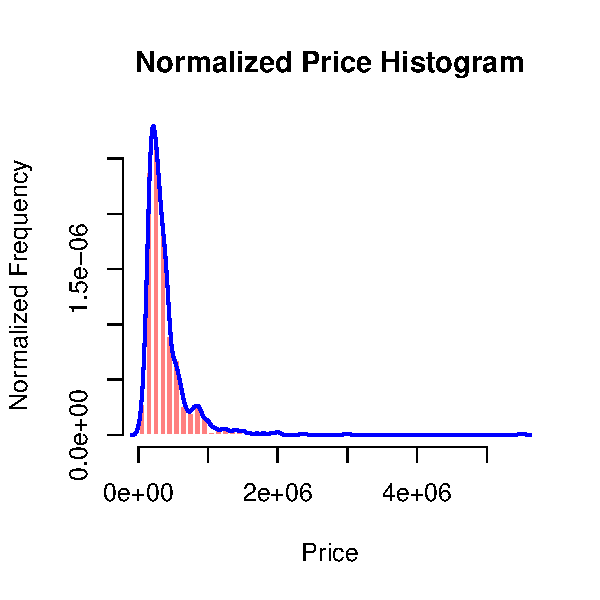
\includegraphics[height=51mm]{price_hist}} & 
\begin{enumerate}
\only<1>{\item[] The \emph{probability distribution} of a continuous RV $X$ is given by a function, $p(X)$. The area under $p$ over $(a, b)$ describes the probability of observing values between $X=a$ and $X=b$.
\item[] $p$ is called the \emph{probability density function} (pdf) of $X$.}
\only<2>{\item[] The pdf can provide intuition for how the RV behaves. 
\item[] For example, the pdf gives us a sense of which values are more likely to be observed compared to others.
}
\end{enumerate}}
\only<3->{\imagetop{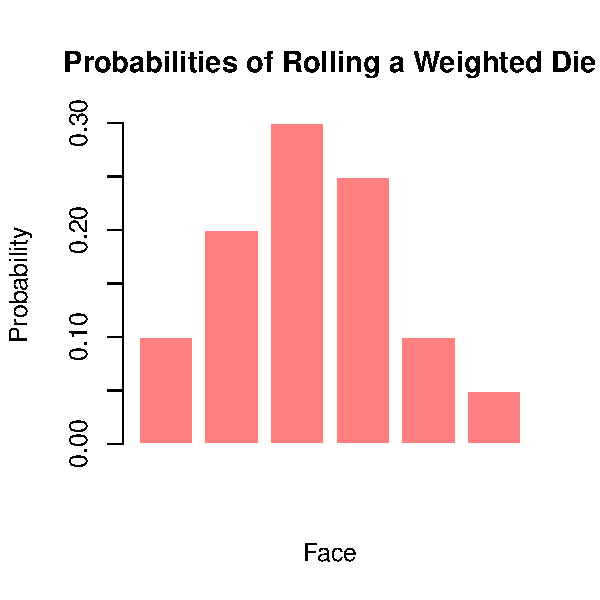
\includegraphics[height=50mm]{die}} & 
\begin{enumerate}
\item[] The \emph{probability distribution} of a discrete RV $X$ is given a function, $p(X)$. $p(a)$, written $p(X=a)$, is the probability of observing $X=a$.
\item[] $p$ is called the \emph{probability density function} (pdf) or the \emph{probability mass function} (pmf) of $X$.
\end{enumerate}}
\end{tabular}

\end{frame}

\begin{frame}{Descriptive Statistics}
For many distributions, we can completely describe the shape of the pdf using just a few quantities. These quantities are usually:
\begin{enumerate}
\item (\textbf{Measuring the `center'}) The \emph{mean} measures the average of the outcomes, weighted by how likely is the each outcome. The \emph{median} divides the area under the pdf into two equal parts.
\item (\textbf{Measuring the `peak'}) The \emph{mode} is the outcome that is the most likely (gives the highest value for the pdf).
\item (\textbf{Measuring the `spread'}) The \emph{variance} is measures the average difference between outcomes and the mean, weighted by how likely is each outcome.
\end{enumerate}
\end{frame}

\begin{frame}{Common Types of Distributions (Continuous)}
\scriptsize
\begin{tabular}{lll}
Normal Distribution& Uniform Distribution& Exponential Distribution\\
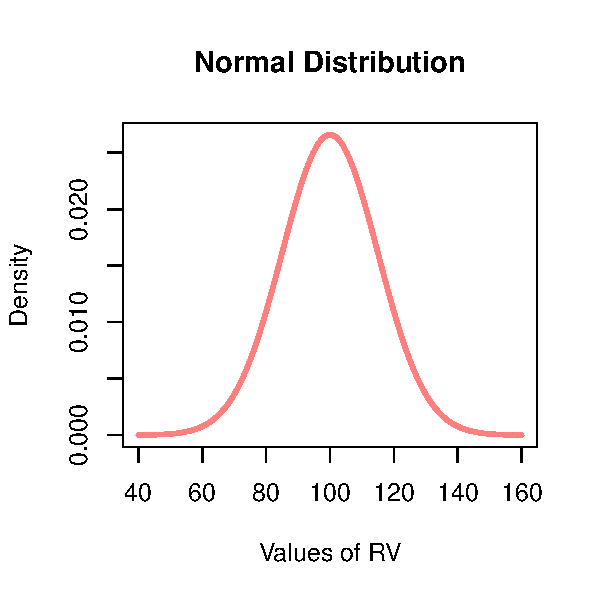
\includegraphics[height=31mm]{dist1} & 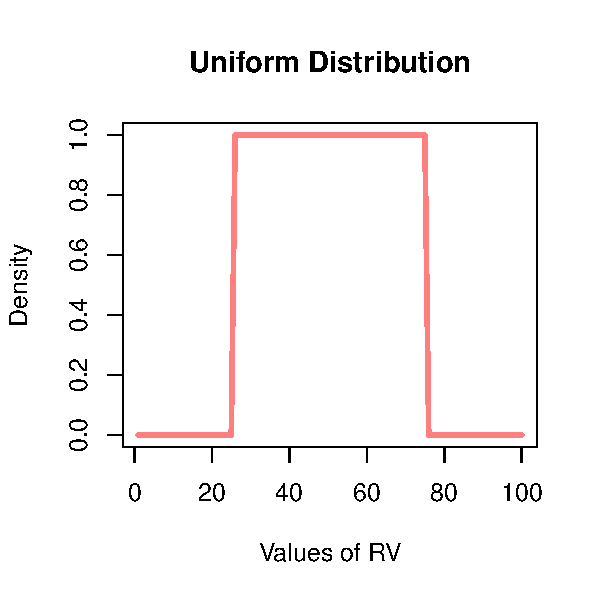
\includegraphics[height=31mm]{dist2} & 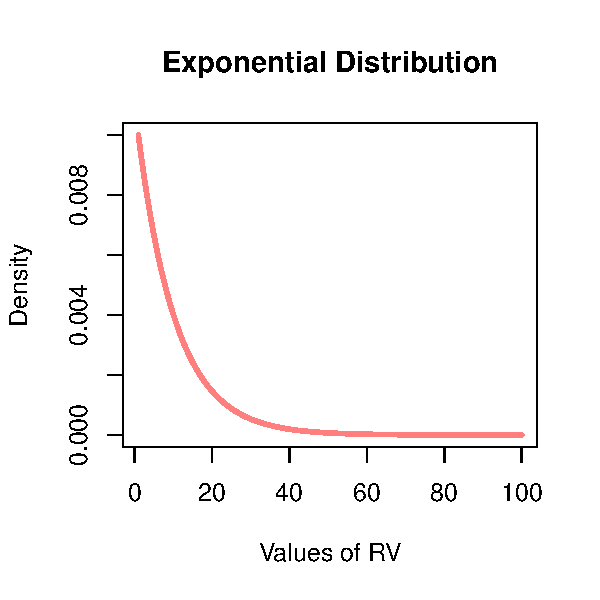
\includegraphics[height=31mm]{dist3}\\
\tiny$p(X) = \frac{1}{\sqrt{2\sigma^2 \pi}} \exp\left\{ -\frac{(X-\mu)^2}{2\sigma^2}\right\}$& \tiny $p(X) = \begin{cases}
\frac{1}{b-a}, &a\leq X\leq b\\
0, &\text{otherwise}
\end{cases}$& \tiny$p(X) = \lambda e^{-\lambda X}$\\
\tiny$\mu\in \mathbb{R}$, $\sigma>0$& \tiny$a, b\in \mathbb{R}$ &\tiny$\lambda >0$\\
\tiny$X\in (-\infty, \infty)$ & \tiny$X\in [a, b]$ & \tiny$X\in [0, \infty)$\\
\tiny$X\sim \mathcal{N}(\mu, \sigma)$ & \tiny$X \sim \mathrm{U}(a, b)$ & \tiny $X\sim \mathrm{Exp}(\lambda)$
\end{tabular}
\end{frame}

\begin{frame}{An Example}
\vskip-0.4cm
\only<1>{Recall that our model for observed housing prices, $P$, given square footage, $A$ is
\[
P = m\cdot A + b + \mathrm{\epsilon}\quad (\text{model for observed prices})
\]
where $\epsilon$ is a random noise variable. 
\vskip0.2cm
What kind of distributions $P | m, b, A, \epsilon$?
\vskip0.2cm
\textbf{Try it yourself:} Come up with a conjecture on the distribution of $P | m, b, A, \epsilon$ by generating values of $\epsilon$ and use them to generate values for $P$.
}

\only<2->{Let's fix $m=1, b=1, A=2$ and choose a normal distribution for $\epsilon$, say $\epsilon\sim \mathcal{N}(0, 1)$. 
\vskip0.2cm
What is the distribution of $P | m, b, A, \epsilon$?
\begin{center}
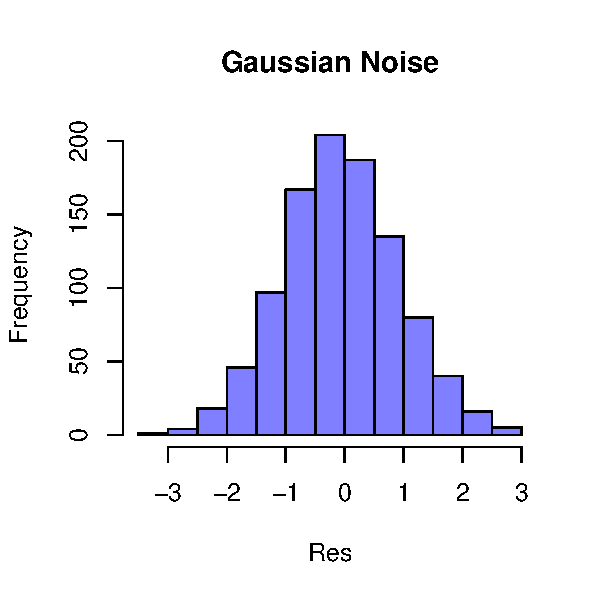
\includegraphics[height=45mm]{noise}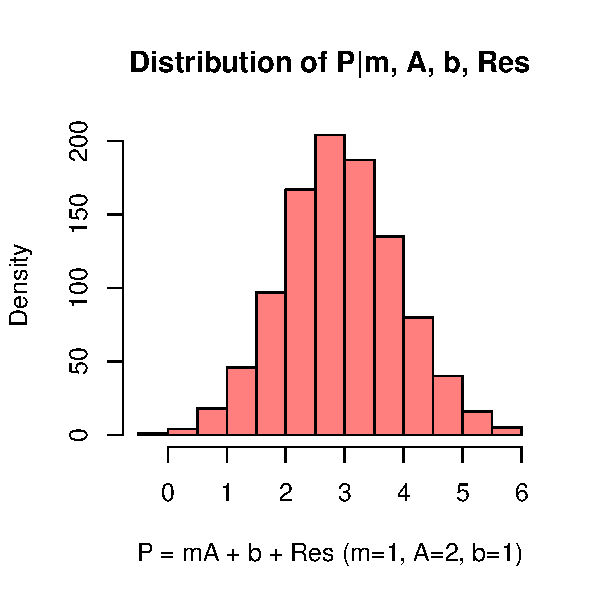
\includegraphics[height=45mm]{cond}
\end{center}
\only<3>{
$P | m, b, A, \epsilon$ looks normally distributed: 
\[
P | m, b, A, \epsilon \sim \mathcal{N}(m\cdot A + b, 1)
\]
}
} 
\end{frame}
%%%%%%%%%%%%%%%%%%%%%%%%%%%%%%%%%%%%%%%%%%%%%%%%%%%%%%%%%%%%%%%%%%%%%%%%%%%%%%
\section{Linear Regression (Univariate)}

\begin{frame}{Back to Our Linear Model}
\only<1>{Recall that our statistical model for observed housing prices is
\[
P = m\cdot A + b + \epsilon
\]
Suppose that $\epsilon \sim \mathcal{N}(0, \sigma^2)$, then 
\[
P | m, b, A, \epsilon \sim \mathcal{N}(m\cdot A + b, \sigma^2).
\]
Can we use this information to find the best linear model for the observed data? 
\vskip0.2cm
\textbf{Try it yourself:} Use $\texttt{python}$ to calculate $p(P | m, b, A, \epsilon)$ for a couple of choices of $m$ and $b$.}
\only<2>{Let's find $m_{MLE}$ and $b_{MLE}$ so that $p(P | m_{MLE}, b_{MLE}, A, \epsilon)$ is maximal. 
\vskip0.2cm
That is, the model $P = m_{MLE}\cdot A + b_{MLE} + \epsilon$ explains the observed data with the highest probability. 
\vskip0.2cm
The above model is called the \emph{maximum likelihood estimator (MLE)}.
}
\end{frame}

\begin{frame}{Ordinary Least Squares}
\vskip-0.4cm
For Gaussian noise, $\epsilon \sim \mathcal{N}(0, 1)$, finding the MLE model is the same as minimizing the MSE loss function!
\vskip0.2cm
Recall, given a set of points $(A_1, P_1), \ldots, (A_n, P_n)$, the MSE of a linear model $P = mA + b$ is 
\[
L(m, b) = \sum_{i=1}^n \left| P_i - (mA_i + b)\right|^2 
\]
$L$ is the lost (or cost) function. Our goal is to \textbf{find $m_{MLE}$ and $b_{MLE}$ such that the lost, $L(m_{MLE}, b_{MLE})$, is minimal}:
\[
(m_{MLE}, b_{MLE}) = \mathrm{argmin}_{m, b} L(m, b).
\]
\end{frame}

%Train/Validation/Test
\begin{frame}{Evaluating Models}
\vskip-0.4cm
\only<1>{Given a set of home listings, we can now fit a maximum likelihood linear model
\[
P = m_{MLE} \cdot A + b_{MLE}
\]
by minimizing the sum of squared residuals (ordinary least squares or OLS). The `error' made by our model in fitting the data is
\[
L(m_{MLE}, b_{MLE}) = \sum_{i=1}^n \left| P_i - (m_{MLE} \cdot A_i + b_{MLE})\right|^2.
\]
This is called the \emph{training error}. 
\vskip0.2cm
But we also need to evaluate our model on new data that it has not yet seen, \emph{test data}.}
\only<2>{
The general process of model fitting and evaluation:
\vskip0.2cm
\begin{enumerate}
\item Given a set of data $(A_1, P_1), \ldots, (A_n, P_n)$, split the data into a \emph{training set} and a \emph{test set}. 
\vskip0.2cm
\item Fit the model on the training set, report error
\vskip0.2cm
\item Fit the model on the testing set, report error
\end{enumerate}
}
\end{frame}


%%%%%%%%%%%%%%%%%%%%%%%%%%%%%%%%%%%%%%%%%%%%%%%%%%%%%%%%%%%%%%%%%%%%%%%%%%%%%%
\section{Linear Regression (Multivariate)}

\begin{frame}{Linear Regression in Multiple Variables}
\vskip-0.4cm
\only<1>{
It's a bit unreasonable for price of a home to depend on square footage alone. In reality, $P$ most likely depends on some combination of square footage, $A$, number of bedrooms $Bd$ and the number of bathrooms $Ba$. 
\vskip0.2cm
The easiest relationship between all 4 variables is again linear
\[
P = a_0 + a_1 A + a_2 Bd + a_3 Ba  + \epsilon.
\]
Again, if we take $\epsilon\sim \mathcal{N}(0,1)$, $P$ (given the model) is a random variable with a normal distribution, $P \sim \mathcal{N}(a_0 + a_1 A + a_2 Bd + a_3 Ba,1)$. 
\vskip0.2cm
Just like before, the values of $a_0, \ldots, a_3$ which maximizes the likelihood of the data (MLE model) can be found by minimizing sum of squared residuals.
}
\only<2>{
When we are fitting a multi-linear regression model 
\[
P = a_0 + a_1 A + a_2 Bd + a_3 Ba  + \epsilon.
\]
to our data. Instead of finding the best fitting line, we find the best fitting \emph{plane}:
\begin{center}
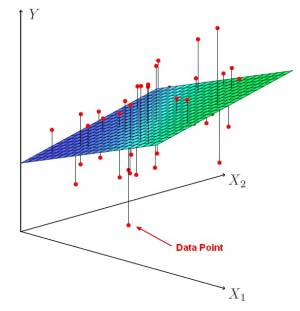
\includegraphics[height=50mm]{multreg}
\end{center}
}
\end{frame}

\begin{frame}{Try It Yourself!}
Try to fit multi-linear models with a few sets of variables other than square footage and report the training and testing errors.
\end{frame}




%%%%%%%%%%%%%%%%%%%%%%%%%%%%%%%%%%%%%%%%%%%%%%%%%%%%%%%%%%%%%%%%%%%%%%%%%%%%%%
\section{Polynomail Regression}
\begin{frame}{Polynomial Regression}
\vskip-0.4cm
As we've noticed, our linear models (univariate and multivariate) don't seem to fit the housing data very well. 
\vskip0.2cm
Maybe this is because the underlying relationship between price and square footage (or number of rooms) isn't linear. Perhaps the model we want is polynomial
\[
P = a_0 + a_1 A + a_2 A^2  + \epsilon,\quad \epsilon \sim \mathcal{N}(0, 1)
\]
\textbf{Note:} our polynomial model is secretly a multi-linear model with two variables, $A$ and $A^2$. 
\end{frame}

\begin{frame}{Try It Yourself!}
Try to fit polynomial model with a few different degrees and report the training and testing errors.
\end{frame}

\begin{frame}{Overfitting}
\vskip-0.4cm
\only<1-7>{One thing we notice immediately was that the error on the training set decreases as the degree of the polynomial increases. 
\vskip0.2cm
So maybe we generally want to pick very high degree polynomials to model our data?
\begin{center}
\only<1>{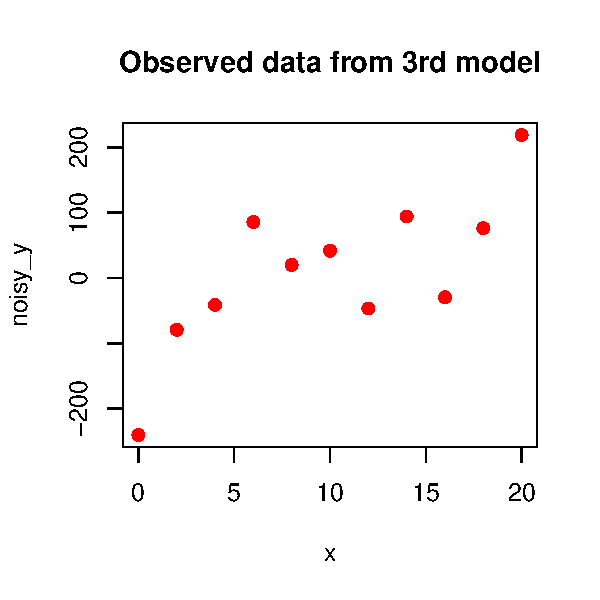
\includegraphics[height=35mm]{scatter_fit}}
\only<2>{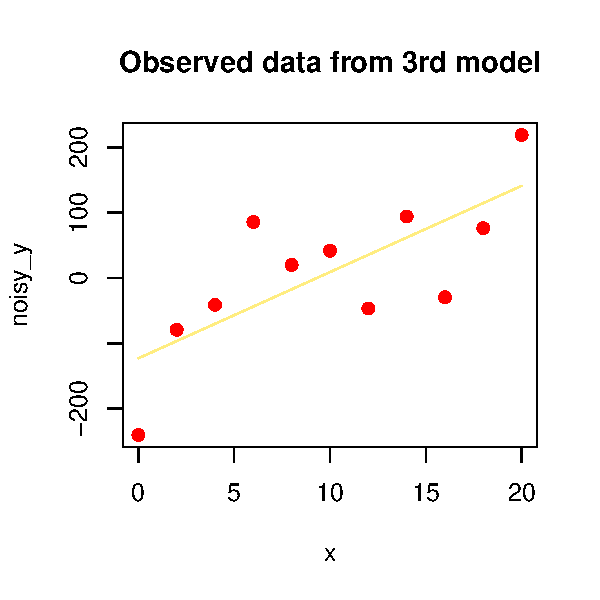
\includegraphics[height=35mm]{deg1}}
\only<3>{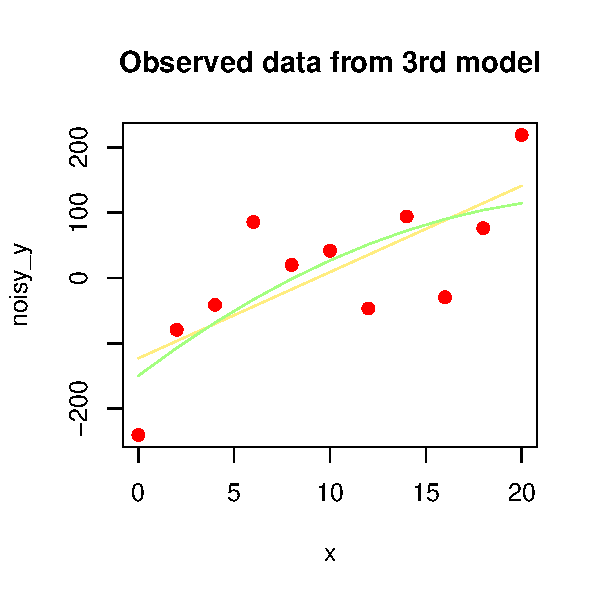
\includegraphics[height=35mm]{deg2}}
\only<4>{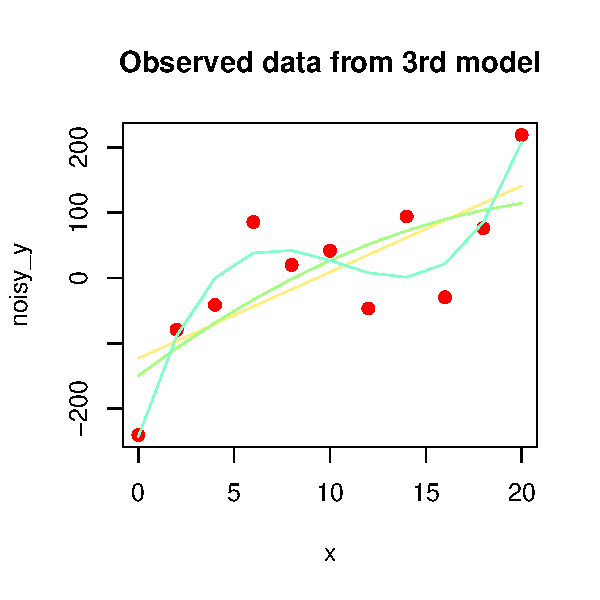
\includegraphics[height=35mm]{deg3}}
\only<5>{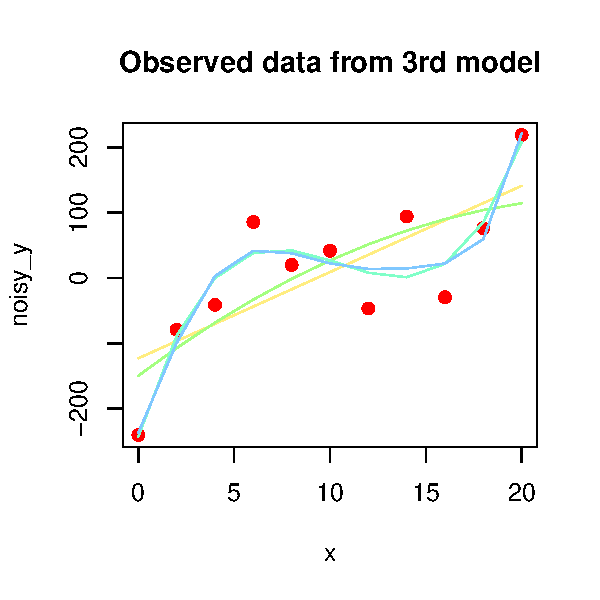
\includegraphics[height=35mm]{deg6}}
\only<6>{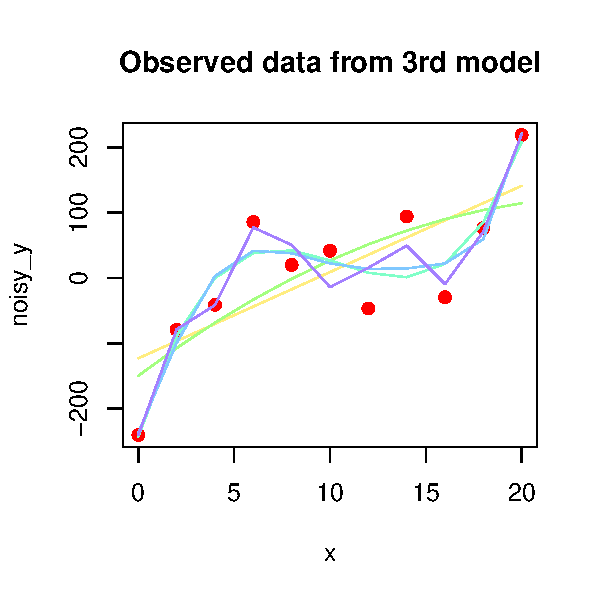
\includegraphics[height=35mm]{deg8}}
\only<7>{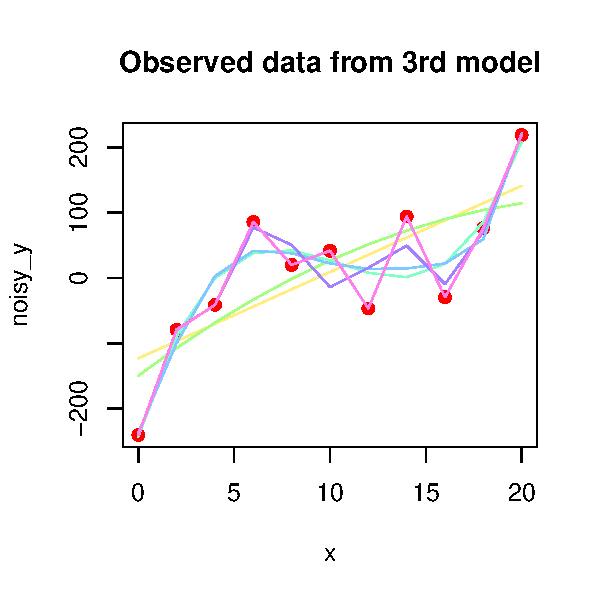
\includegraphics[height=35mm]{deg10}}
\end{center}
What is happening to our model as the degree increases?}
\only<8>{Overfitting can happen with linear regression too!
\begin{center}
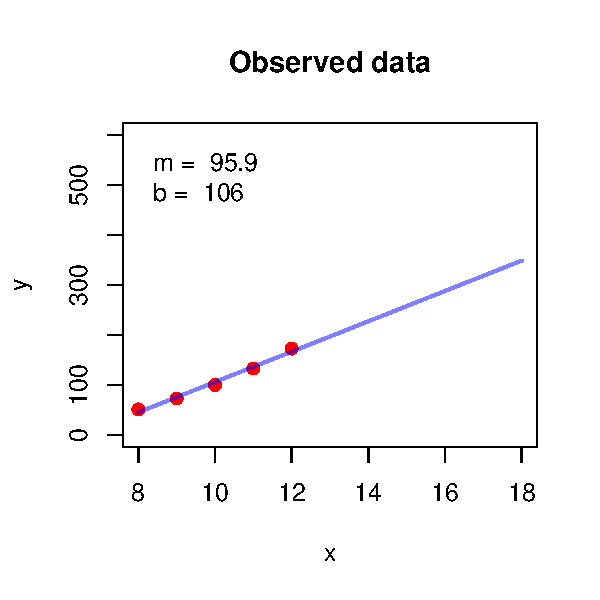
\includegraphics[height=40mm]{linfit1}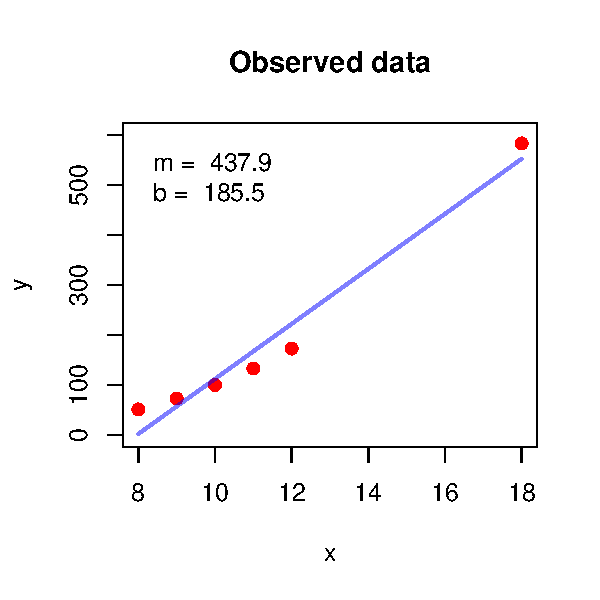
\includegraphics[height=40mm]{linfit2}
\end{center}
\vskip0.2cm
In multiple linear regression, what happens when we have $N$ number of observations and $N$ number of explanatory variables?
}
\only<9>{Overfitting happens when we learn parameters or rules that are too specific to the training set, so much that our model is not useful in explaining new data (we do great on train data but poorly on test).
\vskip0.2cm
Overfitting can happen when we have too few observations compared to the number of variables in our model with which we try to explain the observations.
\vskip0.2cm
Later, we'll see that overfitting can be curbed by regularization and variable selection.
}
\end{frame}


%%%%%%%%%%%%%%%%%%%%%%%%%%%%%%%%%%%%%%%%%%%%%%%%%%%%%%%%%%%%%%%%%%%%%%%%%%%%%%
\section{What is Machine Learning?}
\begin{frame}{Intuition}
The goal of machine learning is to be able to teach machines to make decisions based on previous experience, just like humans.
\vskip0.2cm
\only<1-2>{For example, we give the machine examples of a type of object or scenario. \only<2>{We hope that machine will recognize a new instance of that type of object or scenario.
}
\begin{center}
\only<1>{\includegraphics[height=40mm]{learn_ml}}
\only<2>{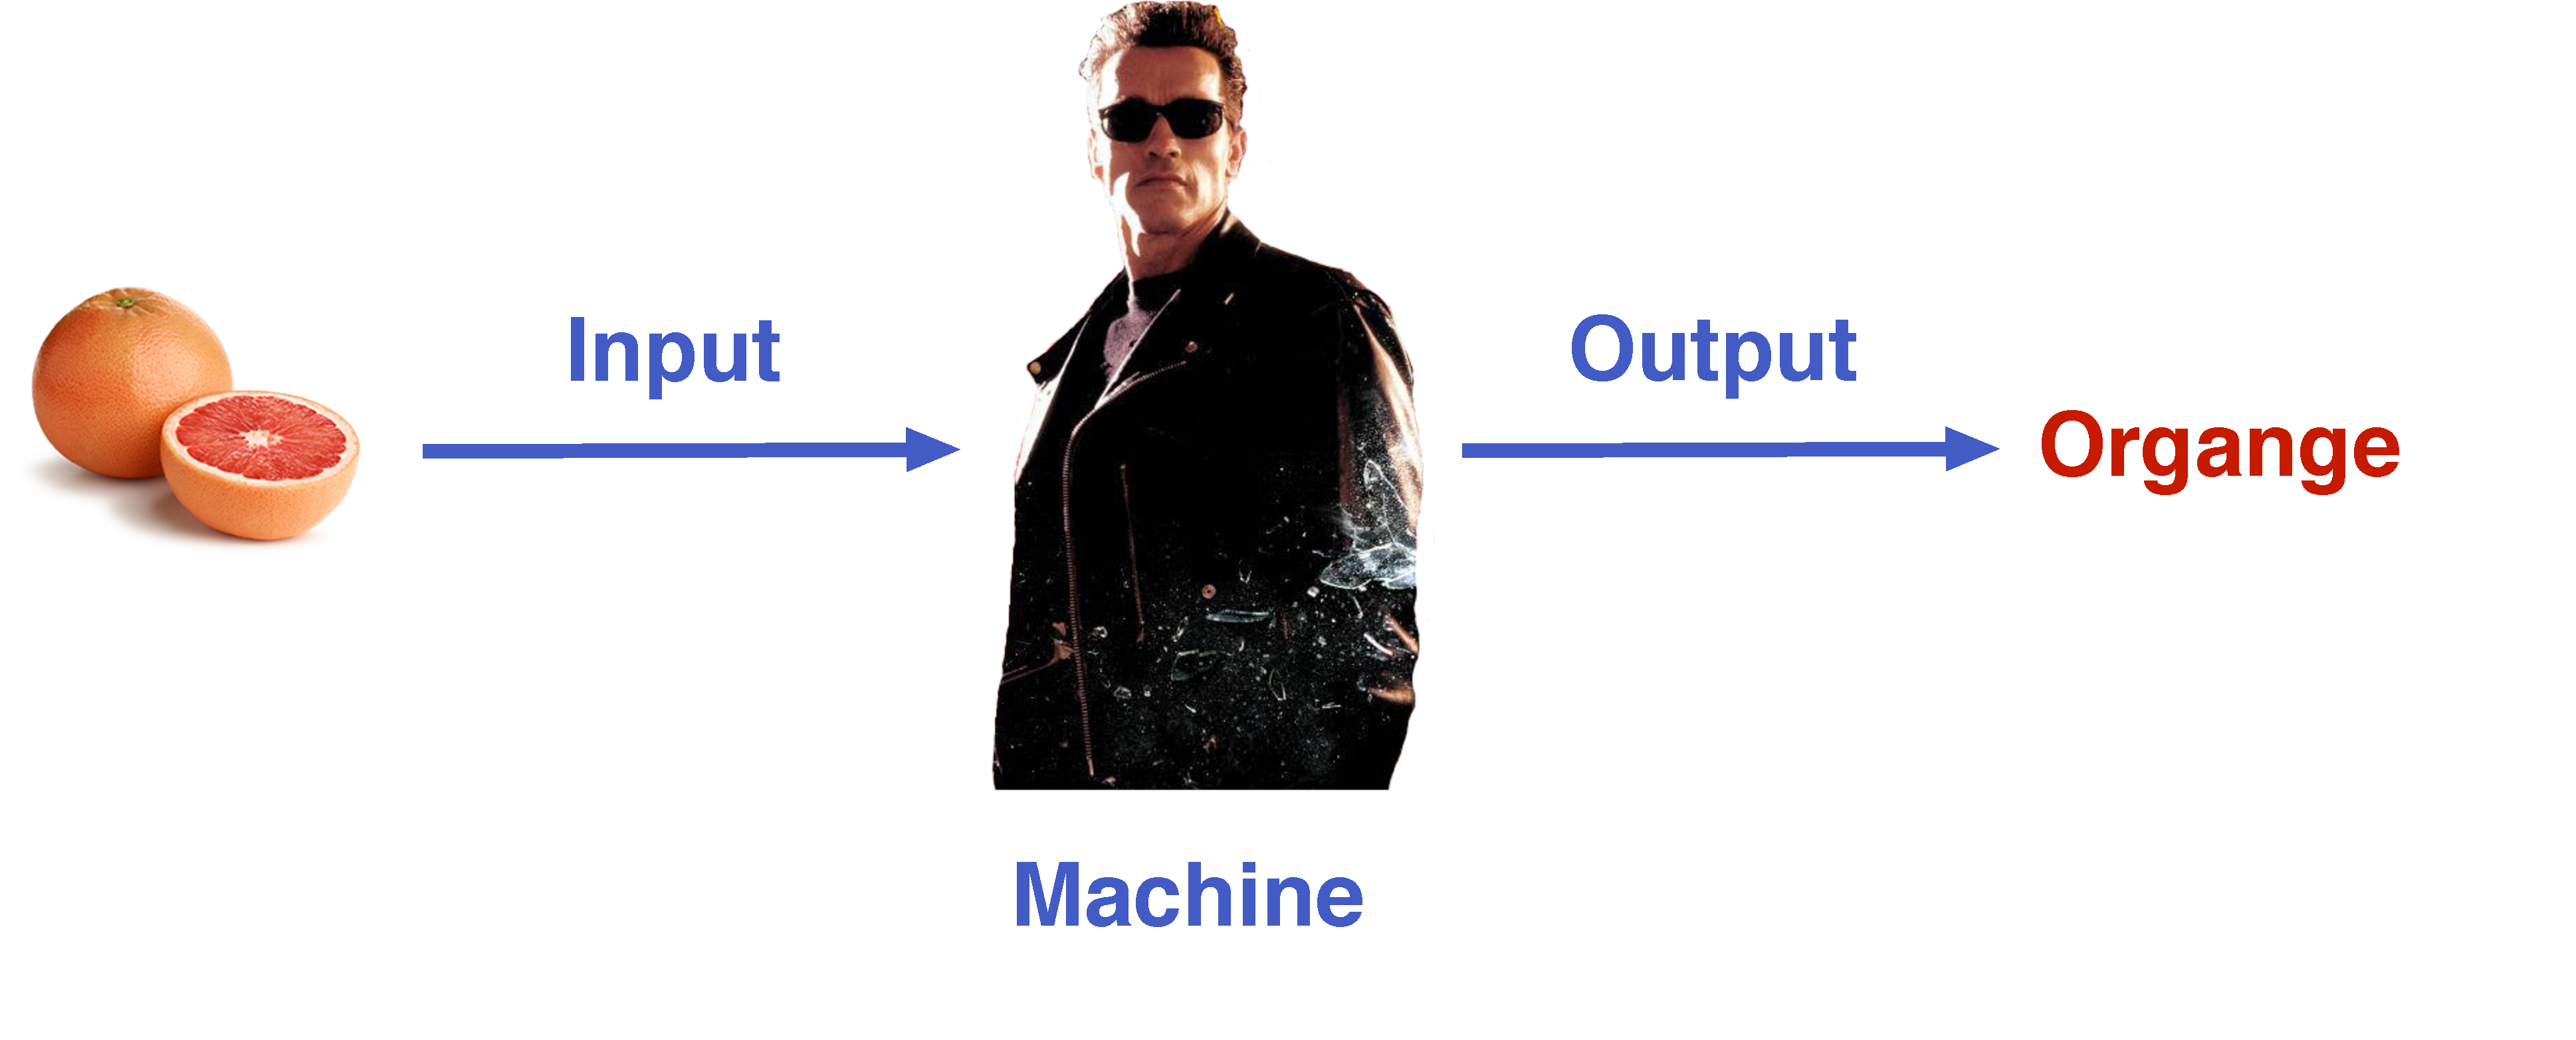
\includegraphics[height=40mm]{pred_ml}}
\end{center}}
\only<3>{The `learning' done by the machine is usually fitting a statistical model to a set of training data. The machine can then use this calibrated model to make decisions when encountering new data.
}
\end{frame}

\begin{frame}{Supervised Learning}
\begin{center}
\only<1>{\includegraphics[height=40mm]{supervise}}
\only<2>{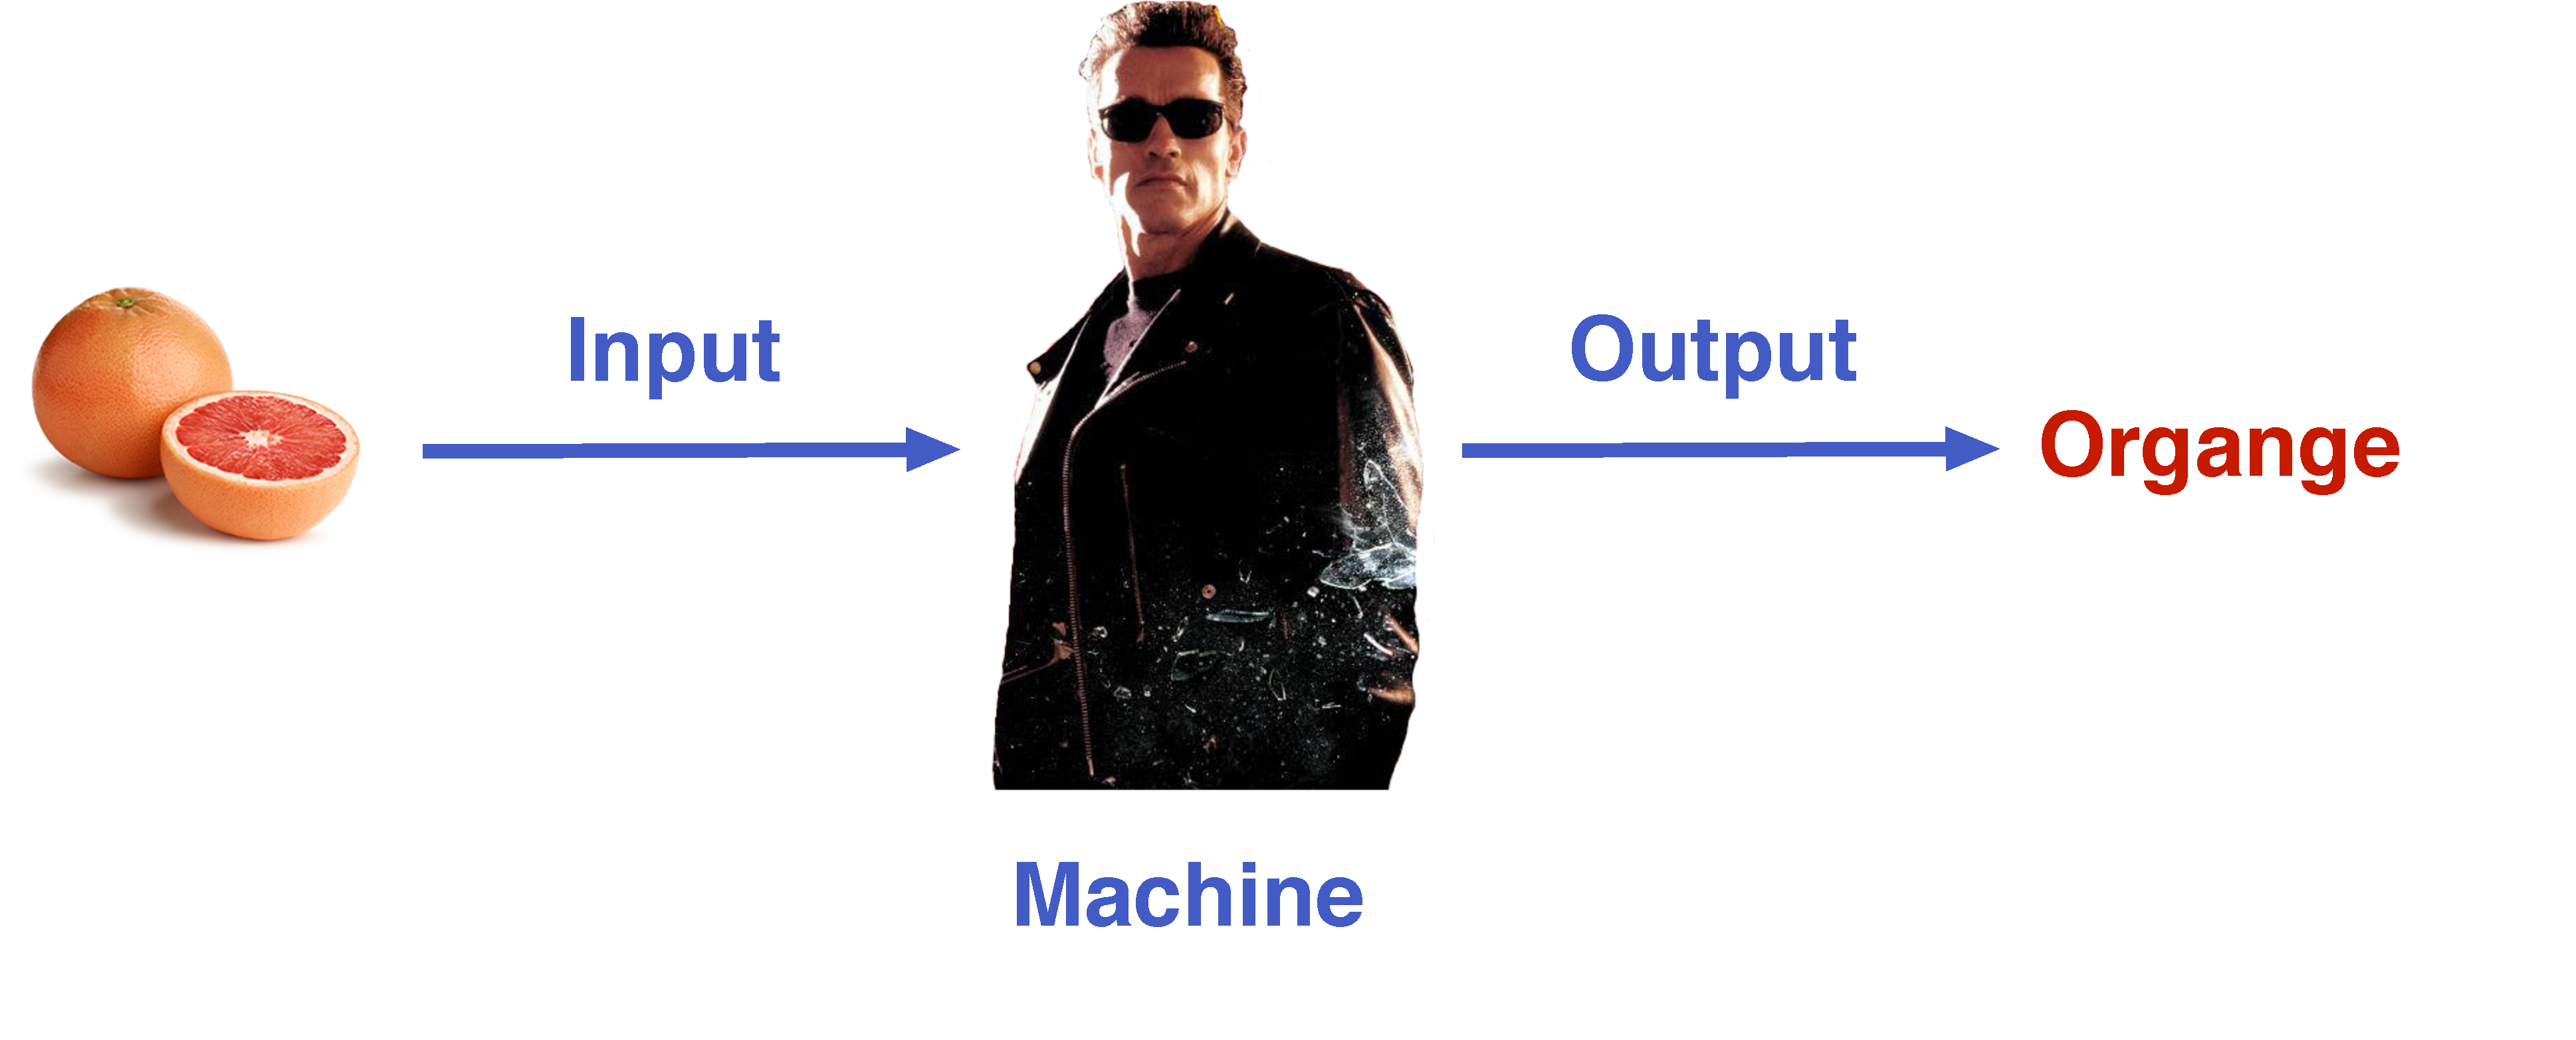
\includegraphics[height=40mm]{pred_ml}}
\end{center}
\end{frame}

\begin{frame}{Unsupervised Learning}
\begin{center}
\only<1>{\includegraphics[height=40mm]{learn_ml}}
\only<2>{\includegraphics[height=30mm]{cluster}}
\only<3>{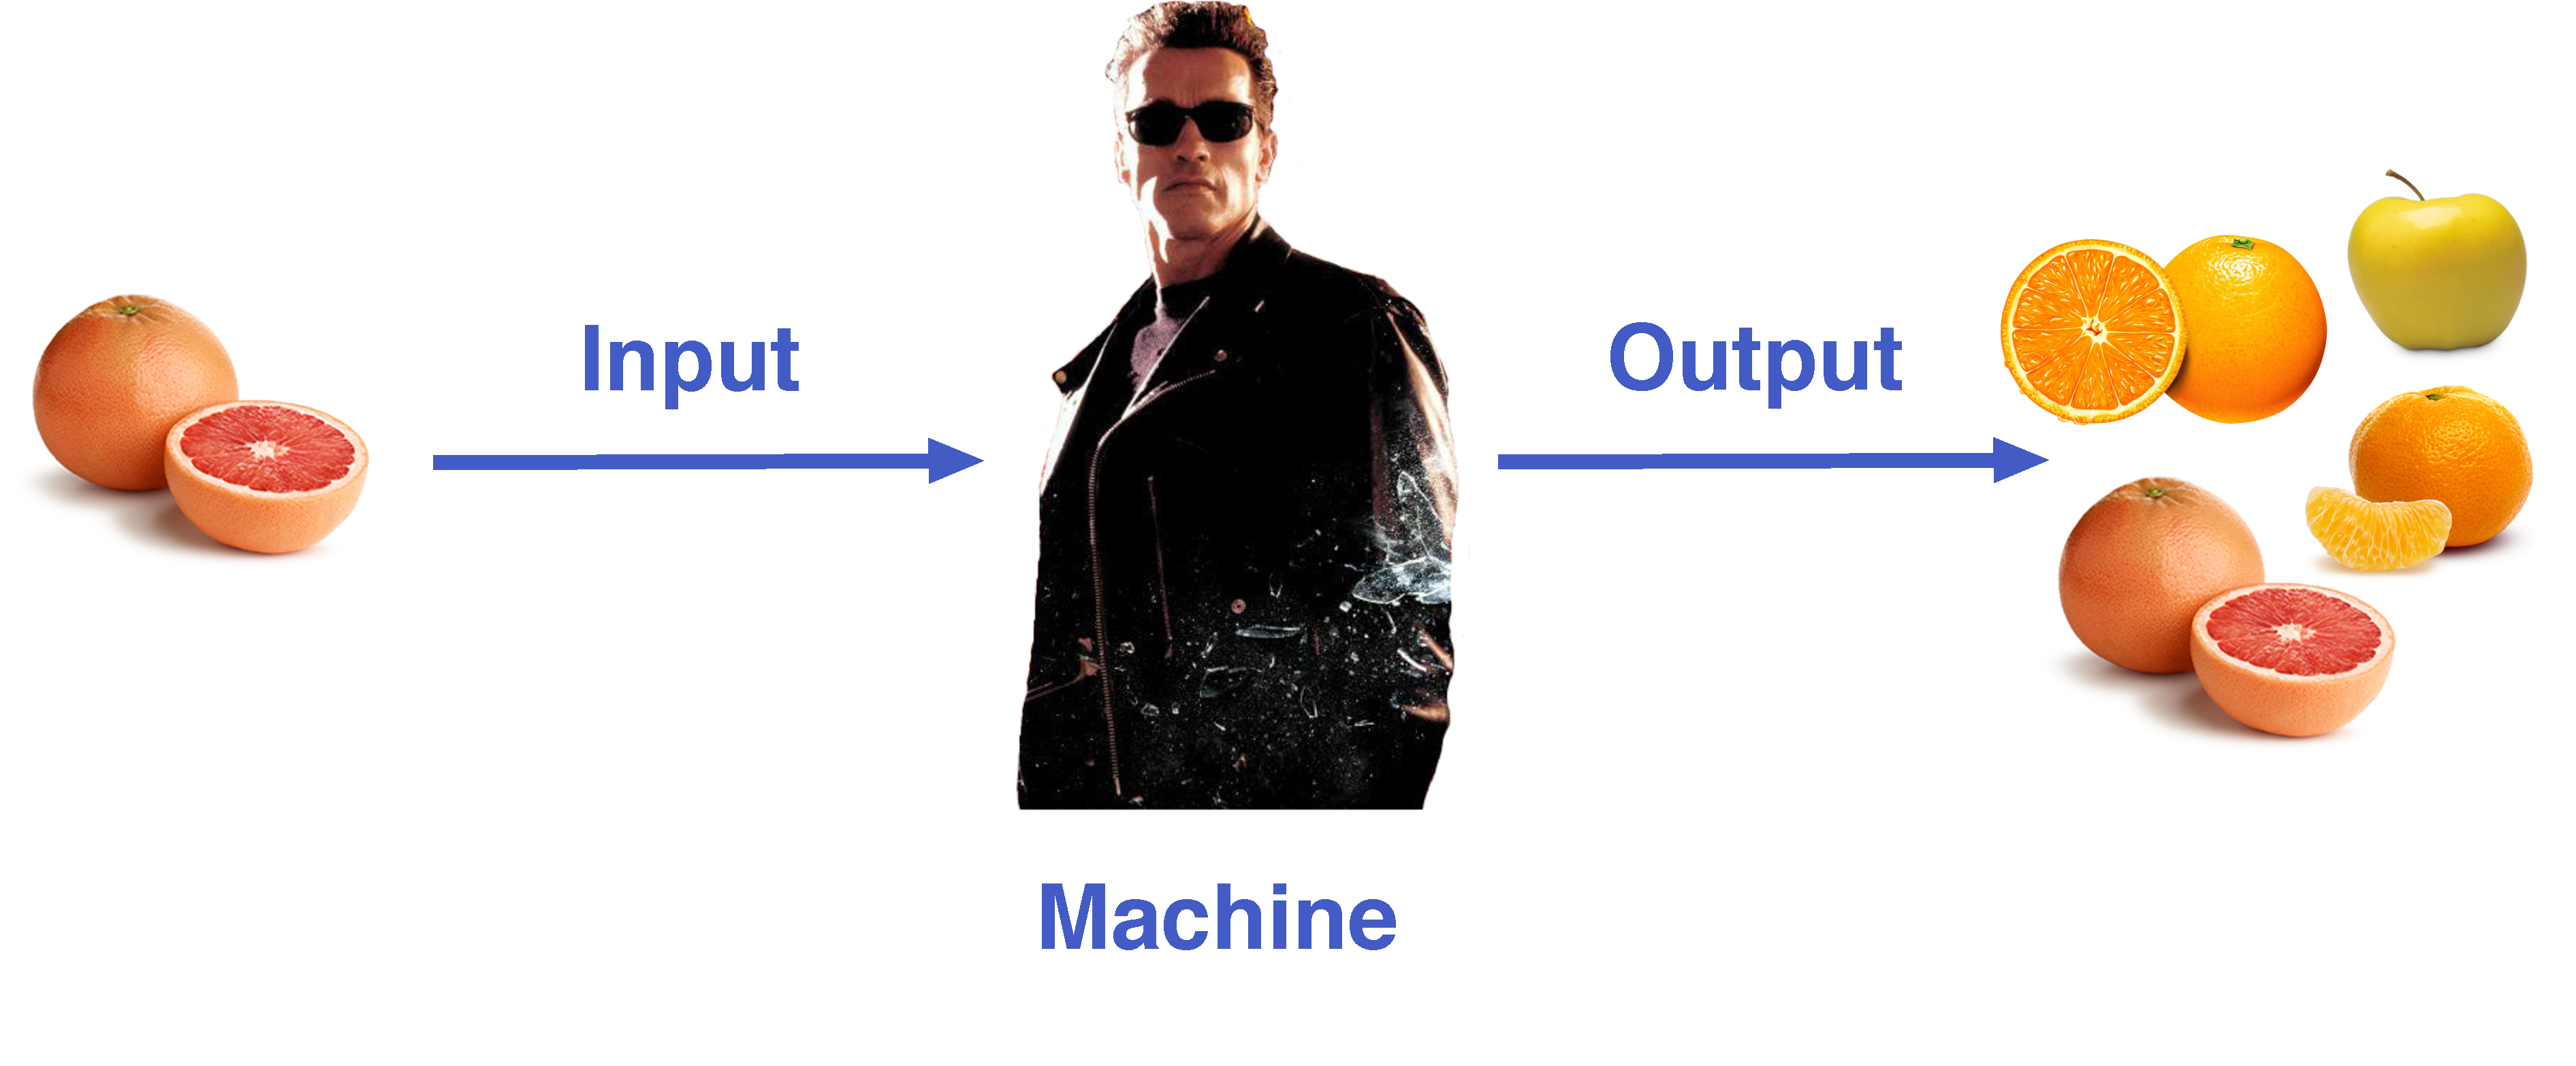
\includegraphics[height=40mm]{unsup}}
\end{center}
\end{frame}

\begin{frame}{Final Thoughts}
\textbf{Question:} What is the difference between machine learning and data science?
\vskip0.2cm
\textbf{Question:} Is regression (linear or polynomial) supervised or unsupervised learning? Why?
\vskip0.2cm
\textbf{Question:} What might be the pros and cons of supervised (resp unsupervised learning)? Why?
\vskip0.2cm
\textbf{Question:} Why is it important to use statistical models in representing data?
\end{frame}

\end{document}
